\section{Physiological Abstraction rules}
\label{abstractionRules}
In the last section we presented a formal model of the human heart as a labeled graph, where each vertex and edge are labeled by a timed automaton.
A given choice of graph structure and of invariant and guard parameters for the automata results in a model that exhibits a given physiological condition, like atrial fibrillation, atrial flutter, etc.
Because a pacemaker is meant to control and improve a range of physiological conditions, there is a need to verify it in a closed loop with all corresponding models.
However this is not possible in practice, since any set of models we explicitly generate will necessarily be incomplete. 
Thus in this section, we present domain-specific abstraction rules that can introduce new behavior to a given model. 
This new behavior is physiologically meaningful and might be manifested by a heart condition not explicitly modeled in the initial set of models.
The physician (or domain expert) remains the ultimate arbiter of what is physiologically meaningful.
Due to space limit we only introduce a subset of abstraction rules. 
The full set is in the technical report [???].

We introduce some notation: given a graph $G$ and an element $x \in V(G) \cup E(G)$ of $G$, we write $A_x$ for the automaton labeling that element.
We write $\Ac(G)$ for the set of automata of a graph: $\Ac(G) = \{A_x : x \in V(G) \cup E(G)\}$.
The set of parameters of the automaton is written $\Pc(A_x) = \{\theta_1^x,\theta_2^x,\ldots\}$. 
Recall that a parameter $\theta$ has both a minimum $\theta_{min}$ (which is used in the guard definitions of the automaton) and a maximum $\theta_{max}$ (which is used in the invariant definition of the automaton).
%The rules are based on the combination of physiological domain knowledge and formal method. %During the rule applications the transition groups incorporated with the models are also merged. These information maintains the physiological meanings of the transitions of the abstract models and are helpful to determine whether the models are appropriate for physiological requirements.%Unlike system modeling in which there is only one concrete system, during environment modeling there are infinite number of environmental conditions that can be generalize by abstractions. In this section, we model the heart as the physiological environment for implantable pacemakers and try to cover different heart conditions and the closed-loop interactions between the heart and the pacemaker. Then using abstraction rules defined over physiological knowledge and principles for over-approximation we construct a series of heart model abstractions with different complexity and coverage. During the rule applications the merging of transition groups are documented thus can be used during model refinements.

\todo[inline]{For each rule, must 

0) give physiological intuition

1) describe the graph to which it applies (could be the whole graph) 

2) describe The conditions on that graph under which it applies (including any assumptions about previously applied rules. Could be empty) 
\\
3) The effect of applying it on both a) the graph (either as pseudo-code or by describing the output graph), and b) the automata 
\\
4) show that is an over-approximation of the relevant behavior (so must define irrelevant behavior)}

%\subsection{Rule 1: Convert Reentry Circuits to Activation Nodes}
Within the conduction network of the heart, there can be multiple pathways between two locations, forming conduction loops. If the timing parameters of the tissue along the loop satisfy certain property, there can be scenarios in which an depolarization wave circling the circuit. The circuits are referred to as \emph{Reentry Circuits}. Since the time interval for an activation wave to circle a reentry circuit is usually less than the intrinsic heart cycle length, the heart rate will be "`hijacked"' by the reentry circuit once the cycling is triggered, causing tachycardia. Reentry is the most common mechanism for tachycardia which can be modeled by our heart models \cite{vhm_embc10}. 

The effect of reentry tachycardia is that activation signals coming out of the circuit with cycle length equals to the sum of conduction delays of the conduction paths forming the circuit. It is therefore reasonable to model a reentry circuit as a self-activation node with the self-activation range equal to the sum of conduction delays. \\
\textbf{Applicable Condition: } The rule only affect the topology of the model therefore can be applied without preliminaries.\\
\textbf{Output graph: }First detect the "essential structure" of the input graph, which are the shortest paths (in terms of conduction delay) connecting self-activation nodes and/or sensing nodes. Then detect all circles in the input graph. For each circle with nodes $N_i,i\in[1\dots n]$ and paths $P_j,j\in[1\dots m]$, remove all "non-essential" nodes and paths, create a node automaton $N_s$ and connect to the nearest sensing node with a path automaton $P_s$.\\
\textbf{Effect on parameters: }For the new node automaton $N_s$, we have :
$$N_s.TERP\_min=min(N_i.TERP\_min), N_s.TERP\_max=max(N_i.TERP\_max)$$
$$N_s.Trest\_min=\sum P_j.Tcond\_min,N_s.Trest\_max=\sum P_j.Tcond\_max$$
For the new path automaton $P_s$, assume the shortest path from $N_s$ to the nearest sensing node has paths $P_k,k\in[1\dots p]$, we have:
$$P_s.Tcond\_min=\sum P_k.Tcond\_min,P_s.Tcond\_max=\sum P_k.Tcond\_max$$
%For more complex structures with multiple circuits, the self-activation range will be the minimum of the shortest circuit to the maximum of the longest circuit. The detailed rule description and implementation can be found in %\cite{regar_tech}.
%\begin{figure}[!h]
%\centering
%\includegraphics[width=0.6\textwidth]{figs/reentry.pdf}
%%\vspace{-5pt}
%\caption{\small Reentry Circuit}
%%\vspace{-15pt}
%\label{fig:reentry}
%\end{figure}

%\subsubsection{Rule 2: Remove Irrelevant Structures}
The network of node and path automata can be viewed as a graph,with nodes as vertices, paths as edges with conduction delay as weight. After the loops within the topology are removed, the topology of the heart model is in form of tree. Within the network there are certain nodes that are more important in terms of model behaviors, we denote them as \emph{Nodes of Interests}, which include:
\begin{itemize}
\item Nodes with self-activations
\item Nodes which interact with the pacemaker
\end{itemize}
Graph algorithm can be performed on the heart model to identify the core structure. Shortest paths can be calculated among nodes of interests. All the nodes and paths along the shortest paths are regarded as core structure. All the other nodes and paths can be then removed without affecting the behaviors of the model. 
%\todo[inline]{Not true. Teh behavior is affected. Because this is a formal methods conference, so behavior and so on mean very specific things.}
\subsubsection{Rule 3: Removing Unnecessary Non-self-activation Nodes}
The effect of non-self-activation nodes is blocking electrical events with interval shorter than its ERP period. If the self-activation nodes at both ends of a core path have self-activation interval longer than the maximum ERP period of nodes along the core path, the nodes can be removed.

For a core path from a self-activation node $N_1$ to another core node $N_2$, for any structure $P_1-N_n-P_2$ which $N_n$ is a non-self-activation node, if $N_n.ERP_{max}<min(N_1.Rest_{min},N_2.Rest_{min})$, replace $P_1-N_n-P_2$ with $P_3$ so that:
$$P_3.cond_{min}=P_1.cond_{min}+P_2.cond_{min}$$
$$P_3.cond_{max}=P_1.cond_{max}+P_2.cond_{max}$$

\subsection{Rule 4: Merge Parameter Ranges}
\textbf{Physiological intuition}. 
The guards and invariants of node automata define timing periods of the heart, like the Effective Refractory Period (ERP) and Rest period. 
By expanding these periods, we introduce new behavior where a heart may stay in rest for longer, or (self-)activate a node faster, or tissue can conduct current sooner, etc.

\textbf{(Sub)graph(s) to which it applies}.
This rules applies to a set of graphs $G_i$ with the same structure (i.e. isomorphic) but possibly with different parameters: $R(G_1,\ldots,G_n) = G'$.
See Fig.[???].

\textbf{Applicability conditions}.
None.

\textbf{Output (sub)graph $G'$}.
$G'$ has same structure as the $G_i$.
Thus $R$ plays the role of an isomorphism between every $G_i$ and $G'$.
Given an element $x$ of $G'$, we abuse notation by writing $R^{-1}(x') = \{x_1,\dots,x_n\}$ is the set of elements that map to it via $R$.

\textbf{Effect on parameters}
Recall Def.~\ref{def:labeledGraph}
For every automaton $A_{x'} \in \Ac(G')$, and every parameter $\theta^{x'}$ of $A_{x'}$, 
\[\theta_{min}^{x'} = \min(\theta^x_{min})_{x \in R^{-1}(x') }\]
\[\theta_{max}^{x'} = \max(\theta^x_{max})_{x \in R^{-1}(x') }\]

\textbf{Proof of abstraction}.
%
%For heart models $H_i,i=[1\dots p]$ with parameter set $\Theta$
%$$\forall i,j,H_a.\theta^j_{min}=min(H_i.\theta^j_{min})$$ 
%$$\forall i,j,H_a.\theta^j_{max}=max(H_i.\theta^j_{max})$$ 
%$H_a$ covers all possible behaviors, thus is an abstraction of $H_i, i\in [1,p]$. The added behaviors in the abstract model do not affect the number of transition groups


%\subsection{Rule 5: Merge Self-activation Nodes with Interaction Nodes}
%%\todo[inline]{not clear}
%The effect of self-activation nodes on the interaction of the pacemaker is triggering sensing events within certain delay. In this rule we merge all the self-activation nodes to their neariest interaction nodes. If there exists multiple self-activation nodes merging to the same interaction node, the parameters of the new model are determined following Rule 3.

\subsection{Rule 6: Replace Blocking With Non-deterministic Conduction}
\textbf{Physiological intuition}. 
\todo[inline]{i don't understand this}

\textbf{Subgraph to which it applies}.
Line graphs with 3 vertices $N_1 P_1 N_2 P_2 N_3$.

\textbf{Applicability conditions}.

\textbf{Output subraph}.
A path $P$ whose path automaton is as shown in Fig?? 

\textbf{Effect on parameters}
$$P.cond_{min}=P_1.cond_{min}+P_2.cond_{min}$$
$$P.cond_{max}=P_1.cond_{max}+P_2.cond_{max}$$
For any self-activation node $N$:
\todo[inline]{what is $N_1$ and what is replacing? what is $N$}
$$N'.rest_{min}=N.ERP_{min}+N.rest_{min}$$
$$N'.rest_{max}=N.ERP_{max}+N.rest_{max}$$


\textbf{Proof of abstraction}.
The effect of a node automaton blocking an activation signal is equivalent to a path not conducting. So we designed new abstract node and path automata $N1$ and $P1$. For any $P_1-N_n-P_2$, it can be replaced by a $P$ with:
\todo[inline]{tshouldn't we see the effect of node ERP somewhere here?}

\begin{figure}[!h]
	\centering
	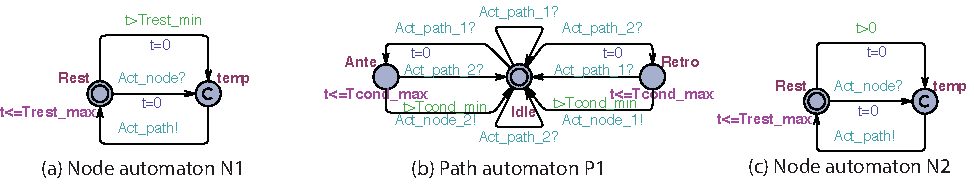
\includegraphics[width=0.9\textwidth]{figs/rule5.pdf}
	%\vspace{-5pt}
	\caption{\small Heart Model Abstractions}
	%\vspace{-15pt}
	\label{fig:rule5}
\end{figure}

\subsection{Rule 7: Replace Conductions With Self-activation}
\textbf{Physiological intuition}. 
This rule applies only after Rule 5 has been applied, and sensing nodes have been merged with self-activation nodes.

The effect of a conduction path is to conduct electrical activity generated by a self-activation node to other nodes. 
If we simply allow all self-activation nodes to activate at any time by setting their Rest period to $+\infty$, we can remove all the conduction paths, while preserving the original behavior (where the Rest period was constrained to a finite interval).

\textbf{Subgraph to which it applies}.
The entire graph $G$.

\textbf{Applicability conditions}.
This rule can only be applied after Rule 5 has been applied.

\textbf{Output subraph}.
All edges are deleted: $G' = (V(G), \emptyset)$.

\textbf{Effect on parameters}
For every node automaton $N$ in $G'$, $N.Trest = +infty$.

\textbf{Proof of abstraction}.

\begin{figure}[!h]
	\centering
	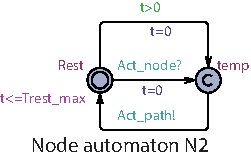
\includegraphics[width=0.3\textwidth]{figs/rule6.pdf}
	%\vspace{-5pt}
	\caption{\small Heart Model Abstractions}
	%\vspace{-15pt}
	\label{fig:rule6}
\end{figure}

\subsection{Heart Model Abstraction Tree}
We first develop a list of concrete heart models corresponding to common heart conditions. 
By systematically applying rules from Section \ref{ruleBasedHeartModelAbstraction} we created an abstraction tree $HM\_tree$ for the heart (\figref{HM_abs}). 
Note that applying rules in different order results different abstraction tree. 
The order used to obtain $HM\_tree$ is based on the domain knowledge that certain heart conditions may have similar behaviors and similar inputs to the pacemaker. 
This systematic grouping maintains the physiological-relevance of the heart model even at higher abstraction levels, and reduce the necessity to resolve ambiguities at lower abstraction levels when model checking certain requirements.
\begin{figure}[!t]
	\centering
	\includegraphics[width=0.9\textwidth]{figs/abs.pdf}
	%\vspace{-5pt}
	\caption{\small Heart Model Abstractions}
	%\vspace{-15pt}
	\label{fig:HM_abs}
\end{figure}

Besides model structure changes, applying abstraction rules also merges the behaviors of the model, which is documented for each abstraction. Here we demonstrate the behavior merging process on a subset of the abstraction tree (\figref{HM_abs}). In $H_{vt}''$, we have self activation behavior $NA.self$ and $NV.self$ for node $NA$ and conduction behavior $NV$,$(NA,AV').cond$ and $(AV',NV).cond$ for path $(NA,AV')$ and $(AV',NV)$. After applying Rule 6 we obtain $H_{vt}''$ with
$$NA'.self=\{NA.self\},NV'.self=\{NV.self\}$$
$$(NA',NV').cond=\{AV'.block,(NA,AV').cond,(AV',NV).cond\}$$
After applying Rule 7 we obtain $H_{all}$ with:
$$NA''.self=\{NA.self,(NA',NV').cond\}$$
$$NV''.self=\{NV.self,(NA',NV').cond\}$$
These information on behavior abstractions are useful to determine whether a model is appropriate for a requirement.
\begin{figure}[!t]
	\centering
	\includegraphics[width=0.5\textwidth]{figs/abs_sim.pdf}
	%\vspace{-5pt}
	\caption{\small Abstraction Example}
	%\vspace{-15pt}
	\label{fig:abs_exam}
\end{figure}
%\subsection{Rule Application Example}
%In this section we demonstrate 
%\todo[inline]{I don't understand what this is...}
%$$NA\_self=\{SA\_self,AVNRT\_self,AF\_self,PAC\_self\}$$
%$$NV\_self=\{PVC\_self,VF\_self,VT\_self\}$$
%$$(NA,AV')\_cond=\{(SA,AV)\_cond\}$$
%$$(AV',NV)\_cond=\{(AV,RBB)\_cond,RBB-RVA\_cond\}$$
%Apply Rule 6:
%$$NA'\_self=\{NA\_self\}$$
%$$NV'\_self=\{NV\_self\}$$
%$$(NA',NV')\_cond=\{AV'\_block,(NA,AV')\_cond,(AV',NV)\_cond\}$$
%Apply Rule 7:
%$$NA''\_self=\{NA'\_self,(NA',NV')\_cond\}$$
%$$NV''\_self=\{NV'\_self,(NA',NV')\_cond\}$$
%\begin{figure}[!t]
%\centering
%\includegraphics[width=0.9\textwidth]{figs/abs.png}
%%\vspace{-5pt}
%\caption{\small Heart Model Abstractions}
%%\vspace{-15pt}
%\label{fig:abs_exam}
%\end{figure}







